\section{Referencia de la Clase Busqueda\-Articulo}
\label{classBusquedaArticulo}\index{BusquedaArticulo@{BusquedaArticulo}}
Permite buscar y seleccionar un art\'{\i}culo.  


{\tt \#include $<$busquedaarticulo.h$>$}

Diagrama de colaboraci\'{o}n para Busqueda\-Articulo:\begin{figure}[H]
\begin{center}
\leavevmode
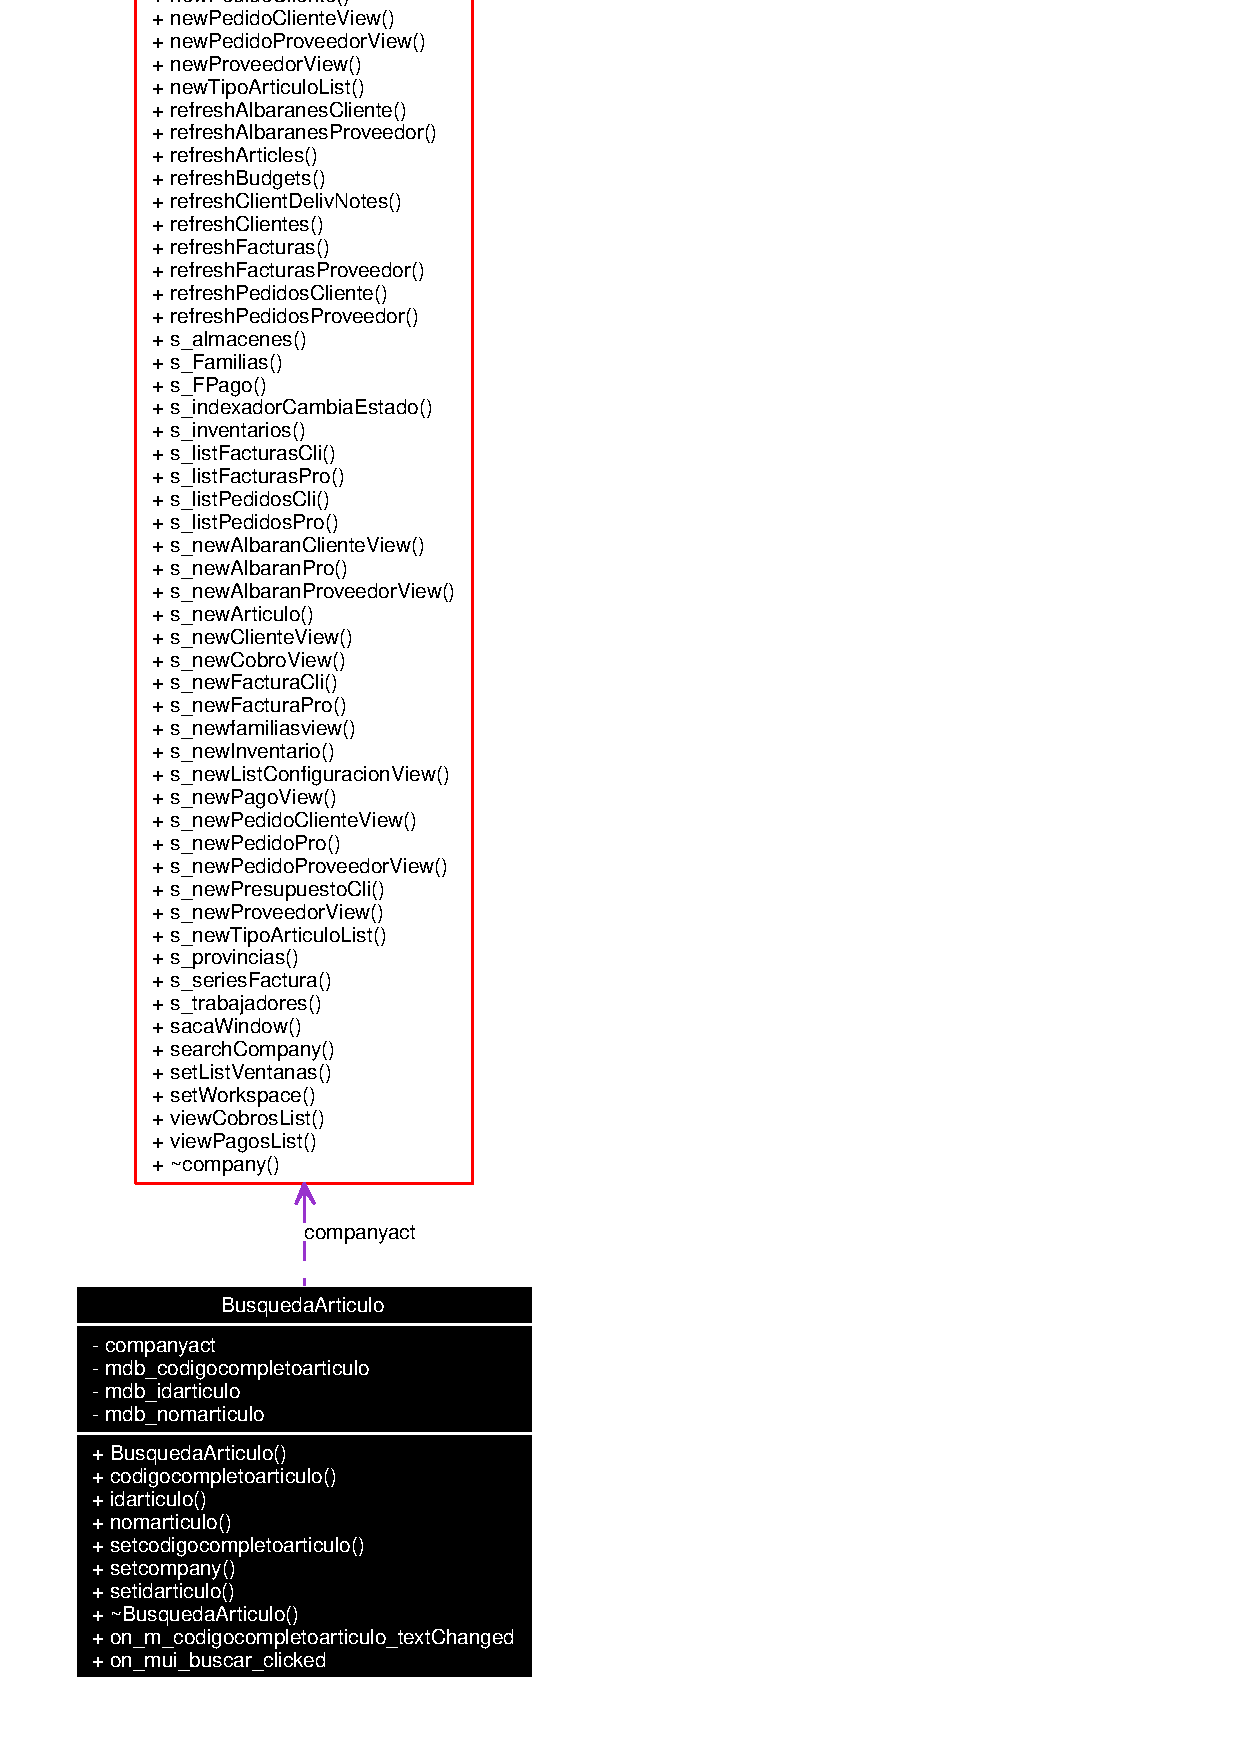
\includegraphics[width=128pt]{classBusquedaArticulo__coll__graph}
\end{center}
\end{figure}
\subsection*{Slots p\'{u}blicos}
\begin{CompactItemize}
\item 
virtual void {\bf on\_\-m\_\-codigocompletoarticulo\_\-text\-Changed} (const QString \&)\label{classBusquedaArticulo_i0}

\item 
virtual void {\bf on\_\-mui\_\-buscar\_\-clicked} ()\label{classBusquedaArticulo_i1}

\begin{CompactList}\small\item\em Busqueda de articulos. \item\end{CompactList}\end{CompactItemize}
\subsection*{Se\~{n}ales}
\begin{CompactItemize}
\item 
void {\bf value\-Changed} (QString)\label{classBusquedaArticulo_l0}

\end{CompactItemize}
\subsection*{M\'{e}todos p\'{u}blicos}
\begin{CompactItemize}
\item 
{\bf Busqueda\-Articulo} (QWidget $\ast$parent=0)\label{classBusquedaArticulo_a0}

\item 
virtual QString {\bf codigocompletoarticulo} ()\label{classBusquedaArticulo_a1}

\item 
virtual QString {\bf idarticulo} ()\label{classBusquedaArticulo_a2}

\item 
virtual QString {\bf nomarticulo} ()\label{classBusquedaArticulo_a3}

\item 
virtual void {\bf setcodigocompletoarticulo} (QString val)\label{classBusquedaArticulo_a4}

\item 
void {\bf setcompany} ({\bf company} $\ast$comp)\label{classBusquedaArticulo_a5}

\item 
virtual void {\bf setidarticulo} (QString val)\label{classBusquedaArticulo_a6}

\end{CompactItemize}


\subsection{Descripci\'{o}n detallada}
Permite buscar y seleccionar un art\'{\i}culo. 

Muestra la parte del formulario que permite buscar y seleccionar un art\'{\i}culo. 



La documentaci\'{o}n para esta clase fu\'{e} generada a partir de los siguientes archivos:\begin{CompactItemize}
\item 
busquedaarticulo.h\item 
busquedaarticulo.cpp\end{CompactItemize}
